\documentclass{beamer}

\mode<presentation>
\usepackage{amsmath,amssymb,mathtools}
\usepackage{textcomp}
\usepackage{gensymb}
\usepackage{adjustbox}
\usepackage{subcaption}
\usepackage{enumitem}
\usepackage[utf8]{inputenc}
\usepackage{amssymb}
\usepackage{newunicodechar}
\usepackage{enumitem}
\setlist{nosep} % optional: removes vertical gaps
\setlist[enumerate]{label=\arabic*)} % custom numbering if you want

\newunicodechar{√}{$\sqrt{\;}$}
\newunicodechar{✅}{\checkmark}
\newunicodechar{❌}{\texttimes}
\usepackage{multicol}
\usepackage{listings}
\usepackage{url}
\usepackage{graphicx} % <-- needed for images
\def\UrlBreaks{\do\/\do-}

\usetheme{Boadilla}
\usecolortheme{lily}
\setbeamertemplate{footline}{
  \leavevmode%
  \hbox{%
  \begin{beamercolorbox}[wd=\paperwidth,ht=2ex,dp=1ex,right]{author in head/foot}%
    \insertframenumber{} / \inserttotalframenumber\hspace*{2ex}
  \end{beamercolorbox}}%
  \vskip0pt%
}
\setbeamertemplate{navigation symbols}{}

\lstset{
  frame=single,
  breaklines=true,
  columns=fullflexible,
  basicstyle=\ttfamily\tiny   % tiny font so code fits
}

\numberwithin{equation}{section}

% ---- your macros ----
\providecommand{\nCr}[2]{\,^{#1}{#2}}
\providecommand{\nPr}[2]{\,^{#1}P_{#2}}
\providecommand{\mbf}{\mathbf}
\providecommand{\pr}[1]{\ensuremath{\Pr\left(#1\right)}}
\providecommand{\qfunc}[1]{\ensuremath{Q\left(#1\right)}}
\providecommand{\sbrak}[1]{\ensuremath{{}\left[#1\right]}}
\providecommand{\lsbrak}[1]{\ensuremath{{}\left[#1\right.}}
\providecommand{\rsbrak}[1]{\ensuremath{\left.#1\right]}}
\providecommand{\brak}[1]{\ensuremath{\left(#1\right)}}
\providecommand{\lbrak}[1]{\ensuremath{\left(#1\right.}}
\providecommand{\rbrak}[1]{\ensuremath{\left.#1\right)}}
\providecommand{\cbrak}[1]{\ensuremath{\left\{#1\right\}}}
\providecommand{\lcbrak}[1]{\ensuremath{\left\{#1\right.}}
\providecommand{\rcbrak}[1]{\ensuremath{\left.#1\right\}}}
\theoremstyle{remark}
\newtheorem{rem}{Remark}
\newcommand{\sgn}{\mathop{\mathrm{sgn}}}
\providecommand{\abs}[1]{\left\vert#1\right\vert}
\providecommand{\res}[1]{\Res\displaylimits_{#1}}
\providecommand{\norm}[1]{\lVert#1\rVert}
\providecommand{\mtx}[1]{\mathbf{#1}}
\providecommand{\mean}[1]{E\left[ #1 \right]}
\providecommand{\fourier}{\overset{\mathcal{F}}{ \rightleftharpoons}}
\providecommand{\system}{\overset{\mathcal{H}}{ \longleftrightarrow}}
\providecommand{\dec}[2]{\ensuremath{\overset{#1}{\underset{#2}{\gtrless}}}}
\newcommand{\myvec}[1]{\ensuremath{\begin{pmatrix}#1\end{pmatrix}}}
\let\vec\mathbf
% ---------------------

\title{Matgeo Presentation - Problem 9.4.34}
\author{ee25btech11021 - Dhanush sagar}

\begin{document}
	

		




%---------------- Title Page ----------------
\begin{frame}
  \titlepage
\end{frame}

%---------------- Problem Statement ----------------
\begin{frame}{Problem Statement}
Rohan's mother is 26 years older than him. The product of their ages (in years) 3 years from now will be 360. We would like to find Rohan's present age.
\end{frame}

%---------------- Mathematical Formula ----------------
\begin{frame}{solution}

Let the present ages be represented as the vector:
\begin{align}
\vec{x} = \myvec{x \\ y}
\end{align}
where $x$ and $y$ denote Rohan's and his mother's present ages respectively.\\

given,\\
eq 1 :Since the mother is 26 years older than Rohan,
\begin{align}
y = x + 26
\end{align}
eq 2 :The product of their ages three years from now is given as
\begin{align}
(x+3)(y+3) = 360
\end{align}

Expanding the above equation:
\begin{align}
xy + 3x + 3y - 351 = 0
\end{align}

This can be written in quadratic (matrix) form as
\begin{align}
\vec{x}^\top \vec{V} \vec{x} + 2\vec{u}^\top \vec{x} + f = 0
\end{align}
\end{frame}
\begin{frame}{solution}
where
\begin{align}
\vec{V} = \myvec{0 & \tfrac{1}{2} \\[4pt] \tfrac{1}{2} & 0}, \quad
\vec{u} = \myvec{\tfrac{3}{2} \\[4pt] \tfrac{3}{2}}, \quad
f = -351
\end{align}

The line $y = x + 26$ can be expressed parametrically as
\begin{align}
\vec{x} = \vec{h} + \kappa \vec{m}, \quad \kappa \in \mathbb{R}
\end{align}
where
\begin{align}
\vec{h} = \myvec{0 \\ 26}, \quad \vec{m} = \myvec{1 \\ 1}
\end{align}

Substituting $\vec{x} = \vec{h} + \kappa \vec{m}$ in the conic equation:
\begin{align}
(\vec{h} + \kappa\vec{m})^\top \vec{V}(\vec{h} + \kappa\vec{m})
+ 2\vec{u}^\top (\vec{h} + \kappa\vec{m}) + f = 0
\end{align}

Grouping powers of $\kappa$, we get:
\begin{align}
\kappa^2 (\vec{m}^\top \vec{V}\vec{m})
+ 2\kappa\, \vec{m}^\top (\vec{V}\vec{h} + \vec{u})
+ g(\vec{h}) = 0
\end{align}
\end{frame}
\begin{frame}{solution}
where
\begin{align}
g(\vec{h}) = \vec{h}^\top \vec{V}\vec{h} + 2\vec{u}^\top \vec{h} + f
\end{align}

Now compute each term:

\begin{align}
\vec{m}^\top \vec{V}\vec{m} &= 
\myvec{1 & 1}
\myvec{0 & \tfrac{1}{2} \\[4pt] \tfrac{1}{2} & 0}
\myvec{1 \\[4pt] 1}
= 1
\\[6pt]
\vec{V}\vec{h} + \vec{u} &=
\myvec{0 & \tfrac{1}{2} \\[4pt] \tfrac{1}{2} & 0}\myvec{0 \\[4pt] 26}
+ \myvec{\tfrac{3}{2} \\[4pt] \tfrac{3}{2}}
= \myvec{14.5 \\[4pt] 1.5}
\\[6pt]
\vec{m}^\top (\vec{V}\vec{h} + \vec{u}) &= \myvec{1 & 1}\myvec{14.5 \\[4pt] 1.5} = 16
\\[6pt]
g(\vec{h}) &= \vec{h}^\top \vec{V}\vec{h} + 2\vec{u}^\top \vec{h} + f
= 0 + 2(\tfrac{3}{2}\times 26) - 351 = -273
\end{align}
\end{frame}
\begin{frame}{solution}
Substituting these results gives:
\begin{align}
\kappa^2 + 32\kappa - 273 = 0
\end{align}

The general quadratic solution is
\begin{align}
\kappa =
\dfrac{
-\,\vec{m}^\top (\vec{V}\vec{h} + \vec{u})
\pm
\sqrt{
\left[\vec{m}^\top (\vec{V}\vec{h} + \vec{u})\right]^2
- g(\vec{h})\,(\vec{m}^\top \vec{V}\vec{m})
}
}{
\vec{m}^\top \vec{V}\vec{m}
}
\end{align}

Substituting numerical values:
\begin{align}
\kappa =
\dfrac{-16 \pm \sqrt{16^2 - (-273)}}{1}
= -16 \pm \sqrt{529}
= -16 \pm 23
\end{align}

Thus,
\begin{align}
\kappa_1 = -39, \quad \kappa_2 = 7
\end{align}

The intersection points are
\begin{align}
\vec{x}_i = \vec{h} + \kappa_i \vec{m}, \quad i = 1,2
\end{align}
\end{frame}
\begin{frame}{solution}
Hence,
\begin{align}
\vec{x}_1 = \myvec{0 \\ 26} - 39\myvec{1 \\ 1} = \myvec{-39 \\ -13}, \quad
\vec{x}_2 = \myvec{0 \\ 26} + 7\myvec{1 \\ 1} = \myvec{7 \\ 33}
\end{align}

The physically meaningful (non-negative) intersection corresponds to
\begin{align}
\boxed{x = 7, \quad y = 33}
\end{align}

Therefore, Rohan's present age is {7\text{ years}}and his mother's present age is{ 33\text{years}}.

\end{frame}
%---------------- C Source Code ----------------
\begin{frame}[fragile]{C Source Code:}
\begin{verbatim}
#include <stdio.h>
#define N 100
void generate_line(double *x, double *y, int n) {
    for (int i = 0; i < n; i++) {
        x[i] = i;        // x values
        y[i] = x[i] + 26; // y = x + 26
    }
}
void generate_conic(double *x, double *y, int n) {
    for (int i = 0; i < n; i++) {
        x[i] = i + 0.1;      // avoid division by zero
        y[i] = 360.0 / (x[i] + 3.0) - 3.0;
    }
}


\end{verbatim}
\end{frame}

%---------------- Python solve.py ----------------
\begin{frame}[fragile]{Python Script:solve }
\begin{verbatim}
import ctypes
import numpy as np
lib = ctypes.CDLL('./libpoints.so')
N = 100
x_line = np.zeros(N, dtype=np.double)
y_line = np.zeros(N, dtype=np.double)
lib.generate_line.argtypes = [ctypes.POINTER(ctypes.c_double),
                              ctypes.POINTER(ctypes.c_double),
                              ctypes.c_int]
lib.generate_line.restype = None
lib.generate_line(x_line.ctypes.data_as(ctypes.POINTER(ctypes.c_double)),
                  y_line.ctypes.data_as(ctypes.POINTER(ctypes.c_double)),
                  N)
print("Sample points from C library (line):")
for i in range(5):
    print(f"x={x_line[i]}, y={y_line[i]}")
    \end{verbatim}
\end{frame}
\begin{frame}[fragile]{Python Script:solve }
\begin{verbatim}
V = np.array([[0, 0.5],
              [0.5, 0]])
u = np.array([[1.5],
              [1.5]])
f = -351
h = np.array([[0],
              [26]])
m = np.array([[1],
              [1]])
mT_V_m = (m.T @ V @ m)[0,0]
Vh_plus_u = V @ h + u
mT_Vh_plus_u = (m.T @ Vh_plus_u)[0,0]
g_h = (h.T @ V @ h + 2*(u.T @ h) + f)[0,0]
a = mT_V_m
b = 2 * mT_Vh_plus_u
c = g_h
kappa = np.roots([a, b, c])
\end{verbatim}
\end{frame}
\begin{frame}[fragile]{Python Script:solve }
\begin{verbatim}
points = [h + k*m for k in kappa]
for pt in points:
    x_val = pt[0,0]
    y_val = pt[1,0]
    if x_val >= 0 and y_val >= 0:
        rohan_age = x_val
        mother_age = y_val
print(f"\nRohan's present age: {rohan_age} years")
print(f"Mother's present age: {mother_age} years")
np.savez("rohan_points.npz",
         x_line=x_line, y_line=y_line,
         rohan_age=rohan_age, mother_age=mother_age)
\end{verbatim}
\end{frame}



\begin{frame}[fragile]{Python Script: plot }
\begin{verbatim}
import numpy as np
import matplotlib.pyplot as plt
data = np.load("rohan_points.npz")
x_line = data['x_line']
y_line = data['y_line']
rohan_age = data['rohan_age']
mother_age = data['mother_age']
x_conic = np.linspace(0.1, 40, 400)  # avoid x=-3
y_conic = 360 / (x_conic + 3) - 3
plt.figure(figsize=(8,6))
plt.plot(x_line, y_line, label="Line: y = x + 26", color='blue')
plt.plot(x_conic, y_conic, label="Conic: (x+3)(y+3)=360", color='red')
plt.scatter(rohan_age, mother_age, color='green', s=100, label=f"Intersection (x={rohan_age}, y={mother_age})")
plt.xlabel("Rohan's age x")
plt.ylabel("Mother's age y")
plt.title("Rohan's Age Problem - Line and Conic Intersection")
plt.grid(True) plt.legend() plt.show()
\end{verbatim}
\end{frame}


\begin{frame}{Result Plot}
 \begin{figure}[H]
     \centering
     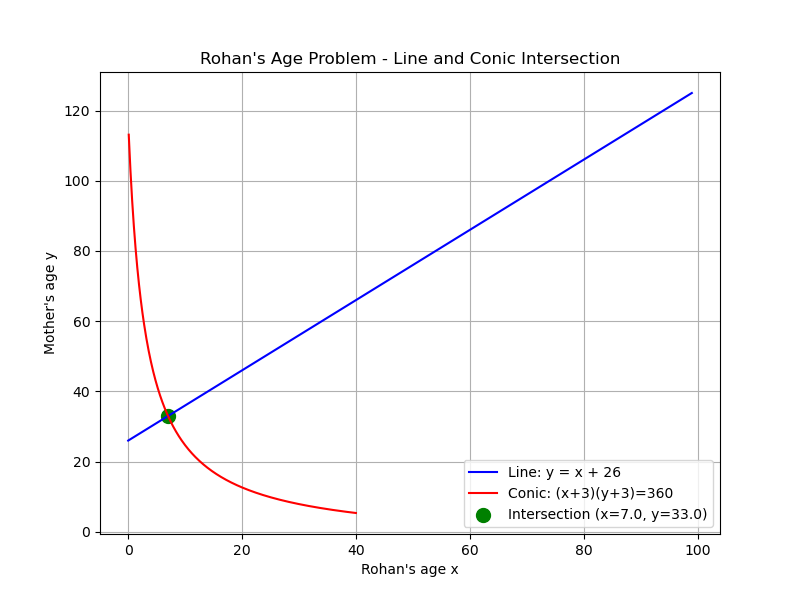
\includegraphics[width=0.8\columnwidth]{Figs/Fig1.png}
     \caption*{}
     \label{fig:fig1}
 \end{figure}
 
\end{frame}
\end{document}
